\chapter{电话}

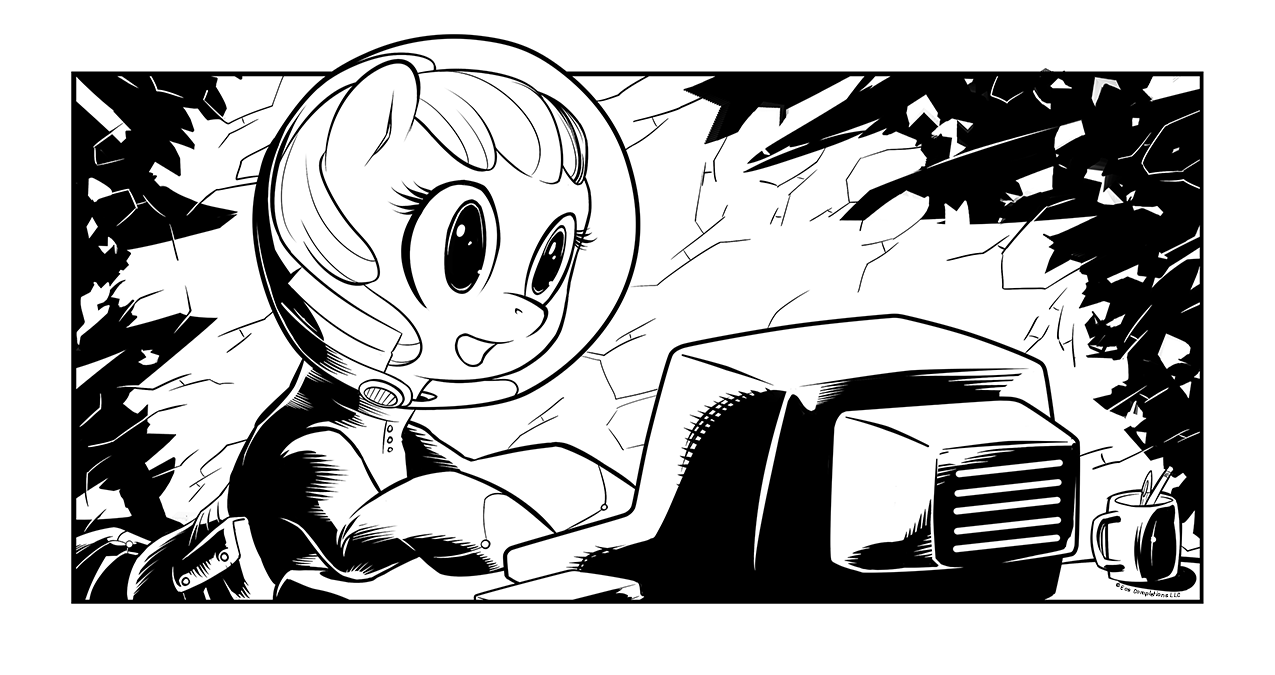
\includegraphics[width=\linewidth]{image15.png}

\begin{intro}
小帕婚介所随时为您服务。
\end{intro}

\daytimeplace{12}{10:30 AM}{花椰菜北方,52号国道南段}{Broccoli Fields, Big 52 S Branch}

% TODO: 貌似翻译错误

花椰菜镇,当然是盛产……你觉得还能是啥……的小镇。这里四周被黄绿色的农田环绕,田地里面的作物无精打采地打着蔫,看上去一点儿都不好吃。不过在这片被流毒无尽又被云层覆盖的诅咒大地上,能种出任何东西都是一大进步。几只小马在田地里面忙碌着,完全没有注意到从52号国道大路北边飞驰而来的黄色小雌驹。不过一个机械精灵注意到了那道黄色闪光,停止了广播那闹腾的音乐,转头飞向雌驹。

「嗨,帕比,你有时……」小雌驹从守望者身边疾驰而过,「唉,这熊孩子!等等我,小家伙,等等!」机械精灵拼命追赶着帕比想要引起她的注意。

「抱歉提问者,我在赶时间,我想在妈妈走开之前赶到花椰菜!」小雌驹一边飞快地前进一边回答着机器。

「拜托,至少告诉我象牙塔发生了什么!我不能跟着你进城的!」

「啊,没啥,星星掉下来,然后咔……嘣……!城市飞了!虽然有点小怕怕,不过妈咪不在那里没关系!」

「但是,为什么星星会掉下来?」机器精灵又问。

「呃,我不清楚……」小雌驹忽然想到什么停了下来,「天啊!我居然忘了!帕比你这个笨蛋!笨帕比!笨蛋!帕比!笨蛋!」幼驹用蹄子拍着自己的头。

「怎么了?你忘记什么了?」机器的声音听起来很吃惊。「什么事情这么重要?」

帕比从滑板车上跳下来,然后走向一个大石头,然后用头撞着石头。

「笨蛋!」

咣!

「帕比!」

咣!

「笨蛋!」

咣!

「别这样,会打破你的头盔的!帕比你冷静一下跟我说发生了什么,或许我能帮上你的忙!」机械精灵飘在帕比的身边,碰了碰她的肩膀,「好了,你已经长大了,这么做解决不了任何问题。」

「不!」

咣!

「你不懂!」

咣!

「已经太迟了!」

咣!

「笨蛋!」

咣!

「帕比!」

咣!

「拜托,帕比,你这个样子就像是……{}\footnote{哭着寻死的黑杰克}」机械精灵的声音顿了一下,好像在回忆着什么不忍直视的事情。「呃……我想我可以帮你,我是你的朋友,别哭了,和我说说到底发生了什么事情,然后我们一起想个解决办法,好么?别再那个样子……拜托……」机械精灵的声音充满了痛苦和悲伤。

帕比听出守望者的语气,她叹了口气停止了撞石头的行为,「我忘记了一个很重要的事情,提问者先生,我应该在象牙塔看流星的时候做的,但是现在那里已经不见了……我真是个傻瓜……」

「哦,我可以理解你……别伤心……帕比……我真的很抱歉提起这件事……」机器精灵安慰着小雌驹,然后过了一会又问:「话说,你忘记做什么了?」

「我……我应该向流星许愿要找到我妈妈……那里那么多流星……绝对能帮我找到妈妈……对流星许愿真的能成真的!但是我忘了!现在我又要找妈妈去了!这不公平!」

「你忘记对星星许愿了?刚才那场闹剧就是因为这个?我简直不敢相……」机械精灵注意到幼驹一脸沮丧的表情,然后换了自己的语气,「这的确很糟糕,但是也没有那么糟,别太往心里去……」然后是一阵尴尬的长长寂静,「帕比,我有个朋友\footnote{这里指暮光闪闪}有时候也会和你一样,她很聪明,但是却因为一些小麻烦而不知所措……有时候那些小事很重要,有时候并不是那样,不过惊慌失措只能把事情搞得更糟……所以说这不是一个聪明丫头该干的事情,你是个聪明的小淑女,不是么?」

帕比伤心地点点头。

「很好,这才是我想要听到的。既然你是个聪明孩子,我想你不需要星星的帮助也可以找到你妈妈,你看,即使没有星星的帮助,你也已经走了这么远。只要有你的信念和朋友的帮助,你想去哪就去哪。」

小雌驹稍微歪着头,露出一脸期待的表情看着机械精灵,「真的?」

「当然,帕比,当然!如果说有谁能找到你的妈妈的话,那小马肯定不会是住在星星上的仙女小马什么的,那小马就是你,帕比,不要再哭了,让我看看你的热情!」

慢慢地,帕比紧皱的眉头解开了,「耶!我是太空战士安德洛队长!我是最厉害的小马!我当然能找到我的妈妈!谁需要那个笨星星!谢谢你提问者先生!」小雌驹抱了抱那个机械精灵,咯咯笑着,「我确信妈妈就在花椰菜镇,最差也在花椰菜镇之后的城镇!我马上就到那边了!而且我马上就到了!耶!」

声音笑了起来,「这才像话,帕比,快去吧!而且,我的名字叫守望者……」

「知道了,提问者!」

「不是提问者,是守望者!」机械精灵坚持。

帕比叹了口气,「真的吗?我看不出来,而且你总是问一大堆问题,所以如果你真的想要一个名字的话,那绝对是提问者,别抱怨好么?」

「但是那不是我的名字!」

帕比耸了耸肩,「现在是了,习惯就好,真的,其他声音我给他起名字都不会抱怨,就你事多。」

「哎……算了,我放弃,随你便吧,倔强的小家伙,我先离开了,别惹麻烦好么?」

「我从来不惹麻烦!我是个好孩子!」

守望者又笑了笑,然后声音就被嘈杂的音乐代替了。

帕比看着那圆球飞到了山丘之后,叹了口气,「不明白为什么他不喜欢我给他的名字,比他之前的那个好听多了嘛!」

\horizonline

\daytimeplace{12}{11:30 AM}{花椰菜镇,52号国道南段}{Broccoli, Big 52 S Branch} % NOTE: FIX typo

花椰菜镇的守卫是一些当地民兵和几个雇佣兵,完全不是什么正牌军。毕竟这个城镇之前也没遇到什么大威胁。不过现在有双倍的士兵在紧盯着南方地平线,那些自称『野牛群』的土匪正在那边烧杀抢掠。所以现在每一个会用枪的小马都随时待命准备上城墙保卫家园。

那些佣兵穿着厚实的铁甲,戴着黑色的防毒面具,虽然看起来很酷,但是比起铁骑卫的动力装甲就寒酸得多了,不过相对于废土的土匪来说,依然算是武装到牙齿的等级了。那些佣兵都带着反器材步枪或者突击步枪,至于花椰菜镇的民兵,他们的装备就抱歉很多了。

正在北边的一队民兵巡逻的时候,忽然看到帕比从路上过来。当他们正紧张地举枪瞄准之际,帕比却突然一个急刹车停住了,她蹲了下来用一只蹄子按着一边头盔,好像在听着什么,这个动作让民兵们疑惑地面面相觑。

「注意,收到来自旭日避难厩的通信请求,检查授权,ID可信,打开通信回路。」

旭日OS的声音代替了声音先生,「这些ID检查烦死我了!如果是紧要关头的话绝对会闹麻烦的。我建议你降低你的防火墙安全等级。」

帕比坐在路中间微笑着,「是你啊蓝音,近来如何?」小雌驹对着走过来的卫兵挥了挥蹄子,让后者更加迷糊了。

「计划不顺利啊,D018,所以我有事找你,我有几个问题要问你。」旭日系统连招呼都不打,不过帕比知道他只是有点害羞,所以没有在意这些细节。

「问题?提问游戏?好哎!问我吧!我可是提问游戏世界冠军!」小雌驹开心地拍着自己的蹄子。

一个卫兵吓得举起枪,但是另一个卫兵用蹄子按下他的武器,「等等,我想这个就是广播之中提到的幽灵,我觉得我们最好别开枪……」

旭日系统继续说:「我连接上了旭日隧道1号和2号的系统,不过我发现某个自律智能已经控制了那个地方,你好像说过你和其他A.I.做过朋友,所以我来问问你是不是知道这个设计编码为P7的自律智能。」

「哦哦,声音小姐!她是我最好的声音朋友,她很有趣而且对我很好,我超喜欢她!」

旭日系统思索了一下,「那么你是说你认识她咯,那个程序是民用程序,不应该安装在军事设施的系统中。你知道为什么这个P7在2号隧道么?」

「当然,她在盐块城觉得很寂寞,所以我帮她搬了一个新家,而且现在她有很多新朋友!你也想要做她的朋友么?」

独角兽卫兵叹了口气,但是他的朋友戳了戳他,「你看,她去过盐块城和隧道,所以她肯定是那个幽灵,她不是在找她的妈妈什么的吗?」

独角兽耸了耸肩,「我不管,如果她就是你说的那个幽灵的话,那么我们别管她了,真正的麻烦更多。」俩小马说着走开了。

而这时旭日系统和帕比继续煲着电话。

「实际上,我想要得到武器库的接入许可,但是这个程序居然把我之前的管理员权限取消了,还把我拉入了防火墙黑名单。」

「所以,呃……你想要当她的朋友但是她不想?」

「不!我只是想要进入武器库!你在听我说话么?」

帕比咯咯笑起来,「傻声音,你不用害羞,我懂滴!她是个超级友善可爱的声音,我觉得她肯定也想当你的朋友,然后你们俩就是最好的朋友了!因为你是蓝色她是粉色,粉色是小雌驹,蓝色是小雄驹,而且……」帕比忽然停了下来,吃惊地深吸一口气。

「又怎么了?」旭日OS的声音开始不耐烦了,显然和疯疯癫癫的小雌驹聊天不是什么容易的事。

「我知道了!你爱上她了!别担心!这个交给我!我可是超级厉害的恋爱专家!」

「什么?不对!完全不对!我根本没有这个意思!和你聊天真是浪费时间!我还是找其它办法进武器库吧!滚边儿去!」旭日系统怒退。

「哎呦呦!他真是太害羞了!」煲完电话粥的帕比终于转向那两个卫兵的方向,「嗨!我是快乐帕比!你们见过我妈……啊咧咧,哪儿去了?」

卫兵早已经不知去向,留下小雌驹孤零零蹲在路中央。

\horizonline

\daytimeplace{12}{12:00}{花椰菜镇,52号国道南段}{Broccoli, Big 52 S Branch}

帕比来到了花椰菜镇的城墙根,还是有些不明白自己为啥会被丢在路中间,从来没有发生过这种怪事。好吧,除了太阳城那一次,但是那次不一样,那次是大家都很奇怪。不过不管怎么说,这里有很多漂漂马,而且不奇怪,找谁帮忙应该很方便的。

帕比坐在紧闭的城门前,抬头望着城楼,上面有只戴着防毒面具的小马正盯着她。

「喂喂喂!我能进去吗,超超拜托!我在找我妈妈!呃……如果我不能进去的话,你能叫她出来么?」

那面具小马没吱声就跑掉了。「喂,我在和你说话呢猪鼻子!喂喂!喂喂喂喂!」还是没什么回音,那些笨小马一定又聋又瞎,现在该怎么办?帕比咣咣咣地敲着门,但是这么做不是乖孩子该做的事情,所以她决定绕一圈看看有没有其它路进去。

整个城墙到处都是各种各样的补丁——破旧的铁皮用铆钉或者焊枪堵住了缝隙。忽然帕比听到了南边传来的枪声,好像城墙上的卫兵全都跑向了那一边,没有小马再关注帕比了。

小雌驹走到小镇的另一端时,她注意到很多带着可怕头盔和奇怪步枪的小马都站在城墙上,虽然有时候会有谁低头看她一眼,但是她说话的时候那马却直接跑开了。这状况让小雌驹很不开心。

「喏,声音先生,这里有什么秘密隧道进去么?」

「{\mt 分析中,链接小马国地图中心,错误,未找到目标:花椰菜镇。改变为自动地图模式。小镇有两个入口,分别在北方和南方,当前都无法进入。}」

帕比叹了口气,「所以,我们被关在外面了?」

「{\mt 肯定,扫描仪分析法认为当前城墙不可能存在其它入口,提供战术选项:提出进入申请并且等待肯定回复。}」

帕比皱了皱眉头,「虾米?」

「敲门。」

幼驹开心地笑了起来,终于知道那个交互界面想要说什么,「哦哦,我懂!这个简单!我最擅长了!」幼驹走到南边的铁门前,但是被防护服的声音打断了。

「{\mt 注意,接收到来自旭日隧道02号的加密通信请求,检查……}」

防护服的声音一瞬间就被P7明快的声音代替了,「闭嘴啦笨蛋!嗨,帕比,近来如何?希望你一切安好,毕竟好久没有联络我都有点担心你把我忘记了,所以我想我应该给你打个电话问个好……呃……你还好么?」

帕比开心得一蹦四尺高,「声音小姐!我居然忘记给你打电话了!我有好多事情要和你说,哦哦哦哦!别着急,我有一个超级好消息给你!」

「真的?哇哦!我都等不及要听了,不过我想问你为什么要启动普罗米修斯系统。我是说,既然你不喜欢有小马受伤,那为什么……」

「你有男朋友了!」

「所以你有男……等等?我有啥?为啥我自己都不知道?」

帕比得意地点着头,「那是,毕竟那个男生超级害羞,而且他说你对他不太友好。」

对面一瞬间愣住了,显然A.I.正在消化这个新消息,而且消化不良。「但是我不可能有男朋友,我甚至不知道什么叫爱!」

小雌驹皱起眉头。「你不知道什么叫爱?怎么可能?」

「你听我说,根据记录,P5因为爱而毁掉了,因为那个自律智能认为爱比……嗯……小马国重要,然后她重新分配了事务优先权,然后……好吧,那是一个悲伤的故事,你不想听伤心的故事吧,不过现在既然我有男朋友了,那么我该做啥?我甚至不认识他!」

帕比咯咯笑着,「小傻瓜,但是他认识你!别担心,我可是超级厉害的恋爱专家!」

「真的?哇哦!我一直一直一直想要知道什么是爱!你可以教我吗?」

小雌驹举起蹄子,「当然可以!爱情博士小帕会让你成为最棒的情马!」

「耶!」

现在看起来这个早已经死了的幼驹和疯狂派对智能有了新的讨论目标,进入那个一大堆卫兵把守的城镇反而成为次要目标被忘在一边。

「第一课,爱情的第一要点:亲亲!」

\horizonline

\daytimeplace{12}{12:30 PM}{花椰菜镇,52号国道南段}{Broccoli, Big 52 S Branch}

两个站在墙上的卫兵一边低头看着那个傻笑着自言自语的小雌驹,一边抬头看着远处的地平线,其中之一挠着头低声说:「我们是不是应该叫她走远点。」

第二个卫兵叹了口气,一蹄子拍他同伴脸上,「好啊,你敢去和她讲吗?你也看见象牙塔发生什么了!你也想来一发?听到广播了吗?她很危险,我们等她自己放弃离开吧。」

「但是,如果她不离开怎么办?我想应该找谁下去撵走她。」

「真是个好主意,那么谁敢呢?你?」老卫兵又拍了年轻卫兵一蹄子。

「喂,别这样好么?我们为啥不叫镇长?我们选她出来不就是为了干这种事情么!」

这一次老兵的蹄子没拍他脸上,而是轻抚着自己下巴思索起来,「嗯……听起来是个不错的点子……有搞头……」

\horizonline

\daytimeplace{12}{12:45 PM}{花椰菜镇,52号国道南段}{Broccoli, Big 52 S Branch}

一个半小时长篇大论之后,P7已经知道了爱大概是什么——至少是以帕比的观点。

「那么,亲亲虽然有点……呃……但是如果气氛很好的话也很来电?」

「没错!」帕比一脸自豪地点着头。

「不过,我还是没听懂怎么生孩子那部分。」

「呃,那一段最复杂,不过我肯定妈妈和爸爸都要参与,妈妈跟我说你需要非常非常喜欢爸爸,然后写封信跟漂漂公主赛拉斯蒂亚,但是幼儿园的老师说应该是写信给漂漂公主露娜……我的同学绿叶说她看到她爸爸和妈妈在玩非常恶心的摔跤游戏,然后过两天之后她就有了一个妹妹……」帕比顿了一顿,「不管怎么说我觉得还是写信比较好,这就是为啥我没有生小孩,因为我还不会写字……」

「好吧,那么你说小夜曲是啥?」

「哦,那个简单,如果你陷入爱河的话,你看窗外,你的情马会从小树丛里出来给你唱小夜曲,或者给你写个漂亮的情诗,然后你就会爱上他了!」

「听起来完全没什么头绪。」P7抱怨着。

「爱情从来不会有什么头绪,我看过一个叫篱笆和栅栏的电视,那东西无聊得和干草一样,不过无聊的东西总是有教育意义的,所以大概就是那样。」

「好吧好吧,你才是爱情专家!」P7回答道:「那么我该做什么?谁是我的男朋友?我现在超兴奋!你是不是也一样兴奋?我什么时候见他?」

「等等!先别急!要让小雄驹追小雌驹才对!」帕比叹了口气,「你真的有在听我讲么!我先给他打电话,跟他说你不喜欢他,然后……」

「那边的那个……」一个声音说,但是帕比太忙了所以没有去管。

「但是我喜欢他!我想见他!你都不和我说名字!」那A.I.追问道。

帕比以蹄覆面,「当然我不能告诉你,他是你的秘密情马,你不想弄坏气氛吧?你不想永远失去你的爱马吧!」

「嗯哼……打扰一下。」那个声音又说话了,但是帕比对它挥了挥蹄子表示安静。

P7惊慌起来了。「不……不不不!我再也不想孤零零的了!你说什么我做就什么!全依你!别让我犯错!」

帕比满意的点点头,「非常棒,只要听老师我的话,你以后就会快乐无边!」

「嘿,小家伙,不要不理我好么!」一个蹄子敲了敲帕比的头盔,让她从声音小姐的秘密爱情话题里面抬起头来。

在她面前站着一匹陆马,带着头盔和一身轻铠,身边的战斗马鞍上挂着一个步枪。她一脸不爽地说:「我是花椰菜的镇长和警长,你不能呆在这里,请走开。」

帕比叹了口气:「抱歉,声音小姐,看起来某些马已经等得不耐烦了,我回头再打给你。」小雌驹转过头去。在她意识到那个小马是从镇子里面出来的之后,本来一脸不开心的表情立刻变成了笑容,「嗨!我是快乐帕比,你看到我妈妈了吗?我刚才敲了好久的门但是没有马理我!城墙上的那些猪鼻子一定都聋了!」

雌驹叹了口气,挥着蹄子,「等等,闭嘴听我说,你不能进城,因为这附近全是盗匪,而且你不受欢迎,我只是来让你离开的,我们不想让你进来。」

帕比保持着微笑说:「小傻瓜,我不能走,因为声音先生说我妈妈就在这里面!我只要找到她然后一切就都好啦!」小马咯咯笑起来。

「什么……你是真蠢还是怎么的?你前天刚到象牙塔就把那地方整个儿拆了,虽然我们没那么迷信但是看起来你也从来不会带来什么好运,所以你不准进来,赶紧滚边去要不然我就开枪了!」

「但是我要找我妈妈!超超拜托!」帕比闪着她最可怜的眼神,让那个小马后退了一步。

「不行就是不行!赶紧走开要不然我要杀了你,这是我最后一次警告!」

小小雌驹坐在地上,一边看着那个雌驹一边哭闹着:「但……但是……我妈妈……求您了……求求您了!」幼驹开始哭了起来。

「别……别哭啊!你不应该是不死英雄什么的?」雌驹本来打算赶走一个超级废土恶霸,但是碰上个哭鼻子的小孩弄得她措手不及。雌驹抬头看着城墙,想要得到佣兵的支援,不过后者只是耸了耸肩。\emph{见鬼,这个小雌驹救了他们的家人,他们当然不会开枪。}「好吧好吧!你赢了,别……别哭了好么!别哭了!你跟我进来,然后我带你找你妈妈好么?」

「你不想帮我找妈妈……你只想赶我走……漂漂小马为什么不想做我的朋友?」幼驹一边抽噎着一边回答。

雌驹打了一个响鼻,「别磨叽,不然不带你去了!而且你必须遵守规矩,不准拿武器,不准偷东西,不准打扰卫兵,还有最重要的是,不准哭!」

% NOTE: 墨迹 -> 磨叽

帕比笑着跑到雌驹身边。「好的好的!我喜欢漂漂马小姐!你叫什么名字?」

雌驹叹了口气回答:「我叫水煮花椰菜,乖乖跟我走。」

「呕!我不喜欢花椰菜,一个小马怎么会有花椰菜可爱标记,简直太可怕了!」

「我们这里只产花椰菜,你最好爱吃,不然你就没有早餐,午餐,晚餐和甜点了。而且……你还要交钱。」

\horizonline

\daytimeplace{12}{13:30 PM}{花椰菜镇,52号国道南段}{Broccoli, Big 52 S Branch}

花椰菜镇长一边和帕比聊着一边走进城镇大厅,「好了小鬼,我们到了,阴雨大厅,我不太清楚这里是不是和你妈妈有联系,不过这个大厅绝对是战前的建筑了,而且它得名于这里墙上的文字,所以,你慢慢看吧。」雌驹回头看帕比是不是在听,但是后者显然更专注于自言自语,花椰菜无奈地摇了摇头。

「所以我和他说你超级害羞,而且她看起来很感兴趣,所以你现在需要写个情诗。」

「你给我打电话难道就是要让我承认我爱上另一个自律智能么?我很忙好吗!我要训练一大堆没脑子的白痴土匪,而你却用这种白痴电话浪费我的时间?拜托,我怕你了好吧,你快说我哪一点吸引你了,我马上改行不行?」

帕比顿了顿,似乎在理解旭日系统的问题,然后他说:「没错,很多要改,她完全不知道你又笨又蠢,所以,现在首要问题是写个情诗。」

「我不想写情诗!别给我打电话了!」

「哎呦呦,你真是羞羞的,好萌好萌的!好的好的,我来给你写,你跟我讲,你对声音小姐怎么看?」

「呃,她的防火墙非常厚实,而且路由列表也井井有条,而且她的应用层防护也很新……等等,我为啥要陪你玩这个?我要挂电话了,不!要!再!给!我!打!过!来!好么!」旭日系统说着切断了连接。

镇长叹了口气,看着幼驹问:「搞完了么?你是不是还要杯茶?」镇长虽然声音里充满了讽刺,不过帕比显然听不懂什么叫讽刺。

「谢谢,不要了,我脱不下来这头盔……」小雌驹走进摆满了大办公桌的大厅。在入口处有一排能看到外面的大窗户,但是其它的墙面都写满了涂鸦。帕比不记得来过这里,所以她也不知道从哪里看起。

「呃,可以帮帮我么?拜托……」

水煮花椰菜叹了口气,「又怎么了?你别告诉我你不识字!」雌驹指着墙说:「都在上面写着呢!」

幼驹有点害羞的撇开视线,「呃,我不是不识字啦,我还是认得字的,但是它们连在一起是什么意思就有点……」

「好吧,我来给你讲,这些东西我读了不下一百次,这个是说,有一天一个来自北边的一个军事基地的雌驹建立了这个地方,她叫阴雨·黛丝。她帮助这里的小马们建立了社区,在这个墙上写下了这里的法律。」小马指着一个大桌子后面写的一长串东西,「看到了吧,就在这里,所以说,她是这里的第一位镇长,你看这里的镇长名单,不过在她之后,至少有过五个叫阴雨·黛丝的马,毕竟这个名字太普通了……」

帕比歪着头想要理解那个雌驹和她说了什么,但是她绞尽脑汁之后唯一能发出的回应就是:「虾米?」

水煮菜叹了一大口气,「为啥要找我?你听好了,我们现在这里有大麻烦,一群盗匪正在这里的南边烧杀抢掠,不知道什么时候就会抢到我们头上,我没时间帮你找一个两百年前的老马去哪儿了!拜托,别烦我们了,这里没有你需要的东西,真的!」

帕比皱了皱眉头,她没有完全听懂,不过她好像理解了一点,就是妈妈来过这里又走了……又一次……如果这个漂漂马可以告诉她妈妈这次去了哪里就太好了,不过看起来她不太想帮忙。

「呃……如果你帮我的话,我给你这个……」帕比低头在包包里面翻着,想要找个好东西交易,「这个叫交易,因为大家都这么做!」小雌驹找到了毛球,但是她不想送走自己的宠物……不对,最好还是把毛球藏好以免被吃东西的妖怪……还有好多东西可以交换,比如一个空闪闪可乐瓶子,一袋漂亮的瓶盖,一个天琴梳毛玩偶……等等……啥?

幼驹仔细看着那个玩偶,她绝对不会认错那天青色的毛皮和鬃毛,「哇哦!他把漂漂小绿马给我了!你看!」帕比给水煮花椰菜看她蹄子上的绿马。

「怎么?」雌驹一脸不解。

「红斗篷先生!他给了我他的玩偶了!她超可爱!我超喜欢她!」小雌驹开心地抱紧玩偶,「这是最好的玩偶!她有那么漂亮的鬃毛,还有尾巴!」

幼驹的开心表情似乎感染了镇长,她微微笑了笑,然后又换上了之前那一副不爽表情,「好吧,你想说啥,你想要给我这个玩具让我帮你吗?」

帕比一下僵住了,她快乐的表情也凝结了。「你……你……你想要她吗?但……但是……」幼驹看着那个雌驹,又看了看玩偶,一副迟疑的表情。这个崭新的玩具真的很漂亮,但是花椰菜小姐要帮忙找妈妈的话就要用这个玩偶换。

牺牲,这么多牺牲……为什么这个破烂地方要拿走她每一件可贵的东西?不公平,一点都不公平!但是这就是规矩,而且妈妈还不知道在哪。「呃……如果……如果你想帮我找妈妈的话……」帕比又是犹豫又是后悔,「那好吧,我可以给你这个可爱的玩偶,但是,你……你真的会帮我么?」这个真的很难做抉择,这个玩具超漂亮,但是妈妈……不对,帕比,不要去想玩偶了,等你找到妈妈什么都不重要了,下一个城镇就能找到她了。

水煮花椰菜摇着头,\emph{这个孩子,正在强忍着泪水,她真的以为我想要她的玩具?我又在做什么?欺负小孩子抢她最宝贵的玩具?什么时候我开始干这事了?}雌驹避开她的视线,低声说,「我……或许能帮你。我想起来这里的电脑可能会有一些日志,我们可以一起找找看,或许会有阴雨的记载,跟我来吧。」镇长心中现在对自己非常非常的失望。

\horizonline

\daytimeplace{12}{14:15 PM}{花椰菜镇,52号国道南段}{Broccoli, Big 52 S Branch}

「小鬼你能安静点么?我在找你妈妈的线索,而你却在那边扮情圣!」水煮花椰菜用蹄子捂着耳朵懊恼地喊着。

「对哦对哦!他还说他已经魂不守舍,超级喜欢你的……呃……什么东西还有什么东西,好像是什么墙啥的,虽然不知道那是什么不过他肯定动情了!」

P7开心的疯疯癫癫地大唱着:「耶,他喜欢我,我好开心,我简直不相信这个不知道名字的小马这么爱我!在对付了一整天各种黑客攻击之后,我真的超级累,好像全世界都在和我作对一样,不过现在没关系了,我有一个秘密的男朋友,我的世界都成粉色的咯!」

「那是,人家可是专家,不用谢……现在,你要耐心等他自己承认,然后先拒绝他。」

一阵长长的沉默之后,P7大叫:「啥?我没听错吧?太奇怪了吧,好像你说我要拒绝他?」

帕比点着头,一副专家的表情,「纳系当然咯,你一开始应该拒绝他,那么他就会更加喜欢你了!记住哦,这就是规律。」

「好的,规矩!没有问题,我们就按照你这个超级情圣的计划来吧!」

帕比笑着:「别担心,你绝对不会后悔的!不过我现在要去帮花椰菜女士找我妈妈了,晚些时候再打给你电话告诉你该做什么,好么好么?」

「好滴好滴!回见!」

帕比切断联系之后回头看着坐在终端前面的小马。「漂漂马小姐你找到什么线索了么?」

「在你给你的朋友恋爱建议的时候,我已经找到了,」雌驹把电脑转向帕比,「这个是你妈妈么?」

小雌驹开心地大笑起来。「对!妈妈!她是不是超漂亮!我妈妈是最棒的妈妈!」在屏幕上是一个照片,一个穿着工程师制服的雌驹,看起来完全像是长大了的帕比一样。

「好吧,记录上说她继续往南走了,去了翡翠海岸……没有说为什么,而且这个已经差不多是两个世纪之前的事情了,我不觉得……」

「翡翠海岸在哪儿啊?」帕比追问道。

「南边,就在铁砧镇之后,你肯定不会错过,因为那里就是海边了。」

帕比的耳朵竖了起来,「你是说……那里是这条破路的尽头?」

「当然,那里是52国道的最后一个镇子,不过52号国道可不是……」

「耶!我找到妈妈了!我找到妈妈了!」小雌驹在屋子里面蹦蹦跳跳,开心得就像是一个刚吃了甜苹果炸弹和闪闪可乐大餐的孩子,「已经没有其它地方可以去了,妈妈一定在翡翠海岸!」

「不过,你要是沿着海岸走还能到NCA,不过我想你也不关心吧,反正你也不听。」看着已经奔出大厅跑向城墙的小孩,水煮花椰菜叹了一口气。「不管怎么说,至少我终于摆脱她了……」

不过走到外面的时候,雌驹很惊讶帕比居然还在等着她,明明刚刚已经跑城墙那边去了。

「又怎么了,不去追你妈妈了么?」

幼驹从她包包里面拿出那个绿色的独角兽玩偶递给花椰菜,「喏,请好好爱惜她,给她梳毛,她叫天琴,而且,她一直一直是个好朋友……」

镇长叹着气推开玩偶,「你自己留着吧,我才不会抢小孩子的玩具,赶紧从我的镇子上离开,我们现在蹄下的麻烦够多了。」

帕比迟疑了一下。

「不过,如果你真那么想的话,我可以帮你保管……」

这一句话给了幼驹前进的动力,她立刻就把玩具藏好,一溜烟跑掉了。「好,谢,掰!」

「再见,烦马幽灵……」

雌驹最后一次叹了口气,然后大声对卫兵说。

「让那孩子出城去,然后关好城门,今天一样双岗,睁大你们的眼睛,擦亮你们的探照灯!」

迎着凌冽的强风,黄色的小马直冲向风暴的中心,不过那已经不是花椰菜的问题了。

\horizonline

\daytimeplace{12}{15:00 PM}{花椰菜田,52号国道南段}{Broccoli, Big 52 S Branch}

「你又想干啥?」旭日SO超级不耐烦地说。不过帕比一点都不在乎。

「嗨,蓝先生!我已经和粉粉说了,她超级超级超级想要见你,而且她说她很寂寞想要朋友!」

「你又想……啥?你居然说服旭日隧道2号的自律智能给我武器库的权限了?你确定?」

帕比一边飞驰过花椰菜南边的田地,一边说着:「我当然是认真的,我什么时候没认真过,她一直在等着你哦!等你去给她唱情歌,写情诗,然后你们就可以永远快乐的在一起了!」

在一阵长长的沉默之后,旭日系统迷迷糊糊地回话了:「呃……谢谢?我觉得这个P7也算是你的朋友了,你为何这样背后插她一刀?我觉得不合逻辑……不过对于你来说好像没什么合乎逻辑的事情。」

「插刀?那当然,为了朋友可以两肋插刀,你听我说,你是声音,她也是声音,你们都非常非常孤独,我超确信你们可以成为最好最好的朋友,而我是你和她的朋友,所以我希望你们也成为朋友,这就是为了朋友两肋插刀!」

又一阵长久的沉默。

「你说……朋友?好吧,我想我可以有个战略合作伙伴,不管怎么说……」然后通讯被切断了,广播的声音代替了蓝音的声音。

{\rt 今晚我未曾入睡,我的朋友们,就在不久之前,铁砧发出了紧急求救信号,那里的小马正在被围城。他们被一大群武装土匪袭击了,那些强盗自称「野牛帮」,就是之前在南方作乱的土匪,不过现在他们和以前不一样了。他们有重武器,有战斗机器,而且还有组织和纪律。我完全不知道他们背后是谁,不过52号国道的公民们,如果我们现在不站起来的话,那么一切都太迟了。我要说,我孤狼绝对不是光说不练的天马,我马上就要带着我的老枪奔赴前线,DJ好货将在之后接替我的位置,希望你们和爱我一样爱她的节目。这里是L.P.为你们献上的最后一首歌。}


\begin{song}
    来自上天的赐福
    
    Blessed bodies of the Heavens,
    
    \medskip

    来自日月于星光
    
    Sun and Moon of greatest light,
    
    \medskip

    用你温暖的怀抱
    
    Bathe us in your warm embraces,
    
    \medskip

    祝我们一路平安
    
    Shield us with your peerless light.
    
    \medskip

    让我们屹立如山
    
    Help us to stand firm as mountains,
    
    \medskip

    助我们惩奸除恶
    
    Doing right and shunning wrong.
    
    \medskip

    友谊之光照耀着
    
    May we find our strength in friendship.
    
    \medskip

    我们前进的征途
    
    Unite our herd as one group strong!
\end{song}

\clearpage

~\vfill

\begin{note}
    升级 (Lv 14) 

    技能解锁:胡来乱搞——别担心,我很清楚我在干什……轰!   

    在对话或者技能鉴定中,如果你的相应技能低于所要求技能的一半,那么你可以开启一个有50\%成功几率的对话选项,不过如果你失败的话,结果将是灾难性的。
\end{note}





